\documentclass{beamer}
\usepackage{Presentation}

\title[Compile-time Deadlock Detection in Rust]{Compile-time Deadlock Detection \\ in Rust using Petri Nets}
\author{Horacio Lisdero Scaffino}
\date{October 9, 2025}
% TWEAK THE FONT SIZE
\setbeamerfont{date}{size=\scriptsize}

\AtBeginSection[]
{
  \begin{frame}{Agenda}
  \footnotesize
    \tableofcontents[currentsection, currentsubsection]
  \end{frame}
}

\begin{document}

\begin{frame}
  \titlepage
\end{frame}

% REMOVE THE LOGO FROM NOW ON %
\logo{}

\begin{frame}{Agenda}
  \tableofcontents
\end{frame}

\section{Introduction}

\subsection{Overview of the tool}

\begin{frame}{A bird's-eye view of the tool}
  The Translator is the core component.
  The model checker and the Rust compiler, \emph{rustc}, are dependencies.

  \begin{figure}
    \centering
    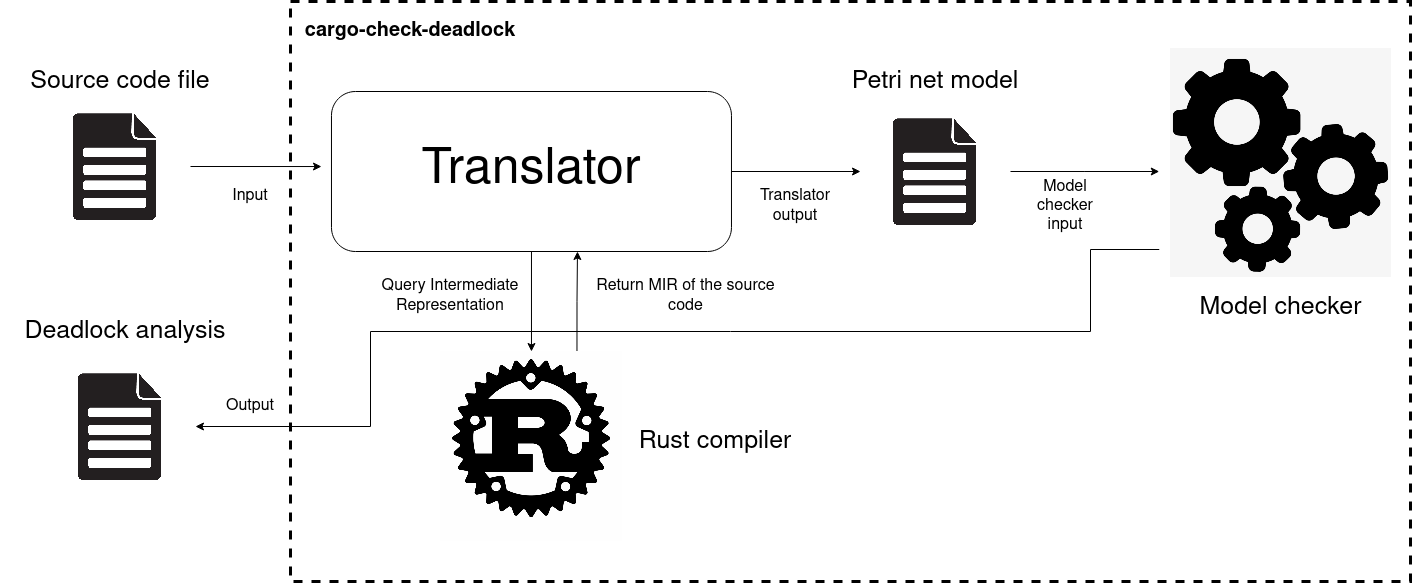
\includegraphics[width=\linewidth]{cargo-check-deadlock-logic-view.png}
  \end{figure}
\end{frame}

\section{Petri nets}

\subsection{What is a Petri net?}

\begin{frame}{Informal definition}
  A Petri net is a mathematical modeling tool
  used to describe and analyze the behavior of concurrent systems.
  It provides a graphical representation of the system's state and its transitions,
  allowing for visual and formal analysis of complex processes.

  \begin{figure}[!htb]
    \centering
    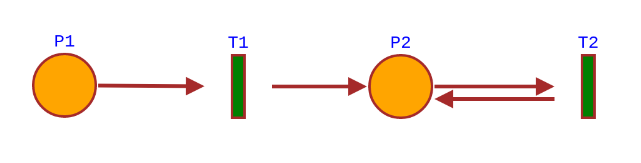
\includegraphics[width=0.8\linewidth]{petri-net-formal-example.png}
  \end{figure}

  \scriptsize
  \begin{itemize}
    \item Places: Represent states in the system (\emph{circles})
    \item Transitions: Represent usually events or actions that occur in the system (\emph{rectangles})
    \item Tokens: Marks inside of places that are created
          and consumed by transitions (\emph{points inside of places})
  \end{itemize}

  \vfill
\end{frame}

\begin{frame}{Mathematical definition}
  A Petri net is a 5-tuple, $ PN = (P, T, F, W, M_{0}) $ where:

  \begin{quote}
    $ P = \{ p_1, p_2, \dots, p_m \} $ is a finite set of places,\\
    $ T = \{ t_1, t_2, \dots, t_n \} $ is a finite set of transitions,\\
    $ F \subseteq (P \times T) \cup (T \times P) $ is a set of arcs (flow relation),\\
    $ W: F \rightarrow \{1, 2, 3, ... \} $ is a weight function for the arcs,\\
    $ M_{0}: P \rightarrow \{0, 1, 2, 3, .... \} $ is the initial marking,\\
    $ P \cap T = \varnothing $ and $ P \cup T \neq \varnothing $
  \end{quote}

  \vfill

  The graph is by definition \emph{bipartite}.
  There can only be edges:
  \begin{itemize}
    \item from places to transitions or
    \item from transitions to places
  \end{itemize}

\end{frame}

\begin{frame}{Transition firing rule}
  \begin{figure}[!htb]
    \centering
    \includesvg[width=0.9\linewidth]{petri-net-transition-example.svg}
  \end{figure}
\end{frame}

\subsection{Examples}

\begin{frame}{Vending machine}
  \scriptsize
  This is a finite-state machine (FSM), a subclass of Petri nets.

  \begin{figure}
    \centering
    \includesvg[width=\linewidth]{state-machine-example.svg}
  \end{figure}
\end{frame}

\begin{frame}{Parallel activities: Fork/Join}
  \scriptsize
  This is a marked graph (MG), a subclass of Petri nets.
  Observe the concurrency between Task 1 and Task 2.
  This cannot be modeled by a single finite-state machine.

  \begin{figure}
    \centering
    \includesvg[width=0.8\linewidth]{parallel-activities-example.svg}
  \end{figure}
\end{frame}

\begin{frame}{Communication protocols: Send with ACK}
  \scriptsize
  A simple protocol in which Process 1 sends messages to Process 2 and
  waits for an acknowledgment to be received before continuing.
  For simplicity, no timeout mechanism was included.

  \begin{figure}
    \centering
    \includesvg[width=0.90\linewidth]{communication-protocols-example.svg}
  \end{figure}
\end{frame}

\begin{frame}{Synchronization control: Readers and writers}
  \scriptsize
  A Petri net system with k processes that either read or write a shared value.

  \begin{itemize}
    \item If one process writes, then no process may read.
    \item If a process is reading, then no process may write.
    \item There can only be zero or one process writing at any given time.
  \end{itemize}

  \begin{figure}
    \centering
    \includesvg[width=0.9\linewidth]{readers-writers-example.svg}
  \end{figure}
\end{frame}

\subsection{Why Petri nets?}

\begin{frame}{Reachability analysis}
  Petri nets can be analyzed using formal methods to conclude whether the net can reach
  a deadlock or not. There is a notion of liveness analogous to the one found in computer systems.

  \vfill
  \pause

  Several model checkers are being developed and
  there is even a Model Checking Contest that takes place every year.
  State-of-the-art tools can handle Petri net models
  with more than \textbf{70 000 transitions} and \textbf{one million places}.

  \vfill
  \pause

  Translating source code to a Petri net has been done before for other programming languages
  \cite{kavi2002modeling,moshtaghi2001} and also for Rust \cite{meyer2020, zhang2022deadlocks}.
  The difficulty lies in supporting more synchronization primitives
  than simple mutexes and translating code from real-world applications.
\end{frame}

\section{Translation}

\subsection{MIR}

\begin{frame}{Compilation stages in \emph{rustc}}
  \scriptsize

  \begin{itemize}
    \item Lexing: The source text is turned into a stream of atomic source code units known as tokens.
          \pause
    \item Parsing: The stream of tokens is converted into an \textbf{Abstract Syntax Tree}.
          \pause
    \item High-level Intermediate Representation (HIR):
          \begin{itemize}
            \scriptsize
            \setbeamertemplate{itemize items}[circle]
            \item Desugar loops: \Rustinline[fontsize=\scriptsize]{while} and \Rustinline[fontsize=\scriptsize]{for} to simple \Rustinline[fontsize=\scriptsize]{loop}.
            \item Type inference: The automatic detection of a type of an expression.
            \item Trait solving: Ensuring that each implementation block (\Rustinline[fontsize=\scriptsize]{impl}) points to a valid trait.
            \item Type checking.
          \end{itemize}
          \pause
    \item Mid-level Intermediate Representation (MIR):
          \begin{itemize}
            \scriptsize
            \setbeamertemplate{itemize items}[circle]
            \item Checking of exhaustiveness of pattern matching.
            \item Desugar method calls to function calls\\
                  (\Rustinline[fontsize=\scriptsize]{x.method(y)} becomes \Rustinline[fontsize=\scriptsize]{Type::method(&x, y)}).
            \item Add implicit dereferencing operations.
            \item Borrow checking.
          \end{itemize}
          \pause
    \item Code generation:
          \begin{itemize}
            \scriptsize
            \setbeamertemplate{itemize items}[circle]
            \item \emph{rustc} relies on LLVM as a backend.
            \item It leverages many optimizations of the LLVM intermediate representation.
            \item LLVM takes over from this point on.
            \item At the end, object files are linked to create an executable.
          \end{itemize}
  \end{itemize}
\end{frame}

\begin{frame}[fragile]{Hello World in MIR}
  \tiny
  BB means ``basic block''. Each one is formed by statements and one terminator statement.
  The terminator statement is the only place where the control flow can jump to another basic block.

  \begin{listing}
    \begin{minted}[fontsize=\scriptsize, frame=none]{Rust}
      fn main() -> () {
          let mut _0: ();                     
          let _1: ();                         
          let mut _2: std::fmt::Arguments<'_>;
          let mut _3: &[&str];                
          let mut _4: &[&str; 1];             
      
          bb0: {
              _4 = const _;                    
              _3 = _4 as &[&str] (Pointer(Unsize));
              _2 = Arguments::<'_>::new_const(move _3) -> bb1;
          }
      
          bb1: {
              _1 = _print(move _2) -> bb2;
          }
      
          bb2: {
              return;
          }
      }      
    \end{minted}
  \end{listing}
\end{frame}

\begin{frame}{MIR as a graph that shows the flow of execution}
  \scriptsize
  The MIR is a form of control flow graph (CFG) used in compilers.
  In this form, the translation to a Petri net becomes evident.

  \begin{figure}[!htb]
    \centering
    \includesvg[width=0.50\linewidth]{mir-cfg-example.svg}
  \end{figure}
\end{frame}

\subsection{Modeling threads}

\begin{frame}[fragile]{Example program}
  Let's consider a trivial program that spawns a thread that does nothing
  and immediately joins it.

  \vfill

  \begin{listing}
    \begin{minted}[fontsize=\scriptsize, frame=none]{Rust}
      fn main() {
        let thread_join_handle = std::thread::spawn(move || {
            // some work here
        });
        // some work here
        let _res = thread_join_handle.join();
      }   
    \end{minted}
  \end{listing}

  \vfill

  \begin{itemize}
    \item \Rustinline{std::thread::spawn} should create an additional token
          that models the program counter of the second thread.
    \item The joining thread should wait until the spawned thread finishes.
  \end{itemize}
\end{frame}

\begin{frame}{Petri net model for a thread}
  \begin{figure}
    \centering
    \includesvg[height=0.85\textheight]{multithreading-example.svg}
  \end{figure}
\end{frame}

\subsection{Modeling mutexes}

\begin{frame}[fragile]{Example program}
  Consider a simple program that locks a mutex twice.
  The second lock operation will deadlock
  because the lock handle returned by the first call to \Rustinline{std::sync::Mutex::lock}
  is not dropped until it falls out of scope.

  \vfill

  \begin{listing}
    \begin{minted}[fontsize=\scriptsize, frame=none]{Rust}
      fn main() {
        let data = std::sync::Mutex::new(0);
        let _d1 = data.lock();
        let _d2 = data.lock(); // cannot lock, since d1 is still active
      }
    \end{minted}
  \end{listing}

  \vfill

  \begin{itemize}
    \item There should be a single place that models the mutex.
    \item Locking the mutex is taking the token from the mutex place.
    \item Unlocking the mutex is setting the token back in the mutex place.
  \end{itemize}
\end{frame}

\begin{frame}{Petri net model for a mutex}
  \begin{figure}
    \centering
    \includesvg[height=0.85\textheight]{mutex-example.svg}
  \end{figure}
\end{frame}

\subsection{Modeling condition variables}

\begin{frame}{How to model a condition variable}
  \begin{figure}
    \centering
    \includesvg[height=0.85\textheight]{condition-variable-model.svg}
  \end{figure}
\end{frame}

\begin{frame}[fragile]{Example program}
  We have to use a very simple example program to keep the net small.
  In this case, the thread is trying to notify itself, which leads to a lost signal.

  \begin{listing}
    \begin{minted}[fontsize=\scriptsize, frame=none]{Rust}
      fn main() {
        let mutex = std::sync::Mutex::new(false);
        let cvar = std::sync::Condvar::new();
        let mutex_guard = mutex.lock().unwrap();
        cvar.notify_one();
        let _result = cvar.wait(mutex_guard);
      }     
    \end{minted}
  \end{listing}

  \begin{itemize}
    \item The model for the condition variable should appear in the Petri net.
    \item The notify place should be set.
    \item But the signal gets consumed because \Rustinline{std::sync::Condvar::wait} was not called.
  \end{itemize}
\end{frame}

\begin{frame}{Petri net model for the example program}
  \begin{figure}
    \centering
    \includesvg[height=0.85\textheight]{condition-variable-example.svg}
  \end{figure}
\end{frame}

\section{Limitations}

\subsection{Limitations of the tool}

\begin{frame}{Limitations of the tool}

  It cannot translate everything possible in Rust / MIR...

  \begin{itemize}
    \item Closures outside of \texttt{thread:spawn} are not supported.
    \item Using arrays, \texttt{Vec}, and other data structures may cause the translation to give false results.
    \item \texttt{Channels}, \texttt{RwLock}, \texttt{Barrier} are not supported.
    \item Async is not supported.
    \item Synchronization mechanisms from external crates such as \texttt{tokio} or \texttt{semaphore} are not supported.
  \end{itemize}
\end{frame}

\subsection{Limitations of the approach}

\begin{frame}{Limitations of the approach}

  Data values are not modelled...

  \begin{itemize}
    \item Deadlocks caused by certain user input
    \item Deadlocks that appear only when a specific number of threads is started
    \item Dynamic code loading and execution
  \end{itemize}

  \vfill
  \pause

  Internals of used crates are not analyzed...

  \begin{itemize}
    \item Deadlocks in calls to libraries or due to them
    \item Deadlocks in \texttt{std} or \texttt{core}
    \item Deadlocks in underlying syscalls
  \end{itemize}

\end{frame}

\section{Bibliography}

\begin{frame}[allowframebreaks]{Bibliography}
  \tiny
  \bibliographystyle{ieeetr}
  \bibliography{
    ../Bibliography/Articles.bib,
    ../Bibliography/Blogs.bib,
    ../Bibliography/Books.bib,
    ../Bibliography/Conferences.bib,
    ../Bibliography/Proceedings.bib
  }
\end{frame}

\section{Additional resources}

\begin{frame}{Online Petri net simulators}
  \begin{itemize}
    \item A simple simulator by Igor Kim can be found on \url{https://petri.hp102.ru/}.
          A tutorial video on Youtube and example nets are included in the tool.
    \item A complement to this is a series of interactive tutorials by Prof. Wil van der Aalst
          at the University of Hamburg. These tutorials are Adobe Flash Player files (with extension \texttt{.swf})
          that modern web browsers cannot execute.
          Luckily, an online Flash emulator like the one found on \url{https://flashplayer.fullstacks.net/?kind=Flash_Emulator}
          can be used to upload the files and execute them.
    \item Another online Petri net editor and simulator is \url{http://www.biregal.com/}.
          The user can draw the net, add the tokens, and then manually fire transitions.
  \end{itemize}
\end{frame}

\begin{frame}{}
  \huge
  \centering
  Questions?
  
  \animategraphics[width=4cm]{10}{Thanks/Thanks-}{0}{6}

  \vfill
  \raggedright
  \normalsize
  \textbf{Links}

  \scriptsize

  \begin{description}
    \item [Tool] \url{https://github.com/hlisdero/cargo-check-deadlock}
    \item [Presentation] \url{https://github.com/hlisdero/thesis/tree/main/presentation_eurorust_2025}
    \item [Published crate] \url{https://crates.io/crates/cargo-check-deadlock}
    \item [Thesis] \url{https://github.com/hlisdero/thesis}
  \end{description}
\end{frame}

\end{document}
